This section details the missing modality feature generation task using a C-MAM. It is split into three parts: the inspiration behind the approach, a high-level explanation of it, and the mathematical formulation and algorithm of the generation task.

\textbf{Cross-modal perceptual associations} describe the cognitive mechanism where variations in one sensory modality evoke responses in another. This phenomenon influences how multimodal information is processed and integrated~\cite{seeing_what_you_hear,Glicksohn2013,Mondloch2004,Spence2011,HAUW2023167,9018269}. An extreme example is synaesthesia, where individuals automatically associate stimuli from one modality with responses in another, such as perceiving specific colours when hearing certain musical notes. A well-known instance of this perceptual filling-in process is illustrated in the silent film \textit{Steamboat Bill, Jr.}, where viewers can imagine the sound of a collapsing house despite the absence of audio (Figure~\ref{fig:steamboat}).
\begin{figure}[htbp!]
    \centering
    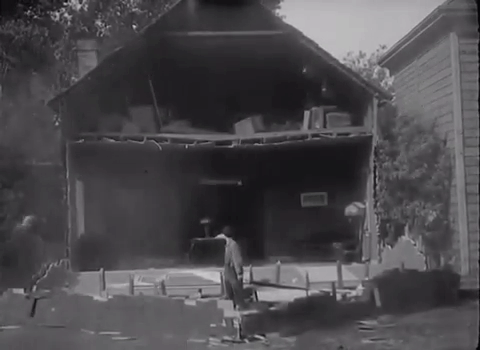
\includegraphics[width=0.25\textwidth]{imgs/steamboat_bill_jr_still.png}
    \caption{The aftermath of the collapsed house. Still taken from the movie [Public Domain] via \href{https://commons.wikimedia.org/wiki/File:GIF_of_Buster_Keaton_in_\%22Steamboat_Bill_Jr\%22_1928.gif}{Wikimedia Commons} }
    \label{fig:steamboat}
\end{figure}

This natural human ability to infer missing sensory information inspires our approach. Similar associations can be learnt within a machine learning framework, allowing a model to infer a missing modality’s features from the remaining available modalities. Rather than modifying or fine-tuning the entire multimodal model, we leverage the pre-trained modality-specific encoders to train a new model, a C-MAM, which generates missing modality embeddings \textbf{without requiring alterations to the original multimodal system.}

\textbf{Learning to Associate} Building on the concept of cross-modal perceptual associations, we apply these ideas to multimodal machine learning. In human perception, different senses interact to compensate for missing information, allowing individuals to infer one sensory input from others. Our approach trains a model to reconstruct missing modality embeddings using the trained encoders of the available modalities, focusing on learning about the model rather than the task being performed by the model.

The proposed \textbf{Cross-Modal Association Models (C-MAMs)} learn associations between available and missing modalities without modifying the multimodal model. Unlike methods that require alterations to the underlying architecture and training procedure, C-MAMs operate \textit{post-hoc}, learning to generate missing modality embeddings from pre-trained encoder outputs. This ensures the trained multimodal model remains unchanged and that C-MAMs are used only when a modality is missing.


\subsection{Problem Formulation}
Multimodal learning improves prediction performance by leveraging multiple data sources like audio, video, and text. However, real-world scenarios often introduce the challenge of \textbf{missing modalities at inference time}, which can significantly degrade model performance. Our objective is to \textbf{reconstruct missing modality embeddings at inference time without modifying the original multimodal model}, ensuring robustness to missing data.

\textbf{Multimodal Learning Framework:} A multimodal dataset consists of $N$ samples, each containing $K$ modalities. Let $M = \{m_1, \dots, m_K\}$ denote the set of input modalities, and let $D = \{(d_1, y_1), \dots, (d_N, y_N)\}$ be the dataset, where each $d_i = \{m_{1_i}, \dots, m_{K_i}\}$ represents the observed modalities, and $y_i \in L$ is the target label. A multimodal model $MM$ learns feature representations through modality-specific encoders $E_m$, $E(d) \mapsto \{f_{m_1}, \dots, f_{m_K}\}, \quad f_{m_i} \in \mathbb{R}^{k_i}$, and fuses them to make predictions, $C(F(f_{m_1}, \dots, f_{m_K})) \mapsto \hat{y}$, where $C$ is the classifier, and $F$ is a fusion function such as concatenation, averaging, or attention-based fusion. The multimodal model is trained using a supervised loss function $\mathcal{L}$, such as cross-entropy or mean absolute error (MAE): $\{\phi_C^*, \phi_E^*\} = \arg\min_{\phi_C, \phi_E} \mathcal{L}(y, \hat{y})$.

\textbf{Challenges of Missing Modalities:} At inference time, one or more modalities may be entirely absent, leading to incomplete inputs. Let \( M' \subset M \) represent the subset of missing modalities, and let \( S = M \setminus M' \) denote the available modalities. The resulting input to the multimodal model is: $d' = d - M', \quad d' = \{ m_i \mid m_i \in S \}$.
This formulation generalises the missing modality scenario to allow for any combination of absent modalities, rather than assuming only one missing modality. Standard multimodal models are not explicitly designed to handle such cases, often relying on the assumption that all modalities are present during inference. A common approach to handling missing modalities is incorporating a reconstruction module within the classification model. For example, autoencoders trained to reconstruct all modalities while jointly optimising for classification~\cite{zhao-etal-2021-missing,redcore}. In these methods, the model is trained to both \textbf{predict the output and reconstruct modality embeddings}, which introduces \textbf{competing objectives}. This can lead to suboptimal representations, as the model must balance classification and reconstruction. Additionally, these methods require modifying the core multimodal model, making them impractical for already deployed systems where retraining is infeasible.

\subsection{Cross-Modal Association Models (C-MAMs)}
To address these limitations, we introduce \textbf{Cross-Modal Association Models (C-MAMs)}, a targeted and modular approach that reconstructs missing modality embeddings without modifying the trained multimodal model. Unlike existing approaches, C-MAMs are \textbf{fully decoupled} from the multimodal model, ensuring that reconstruction does not interfere with classification.

C-MAMs reconstruct missing modality embeddings by leveraging the available modalities' feature representations. Given a missing modality $m'$, the remaining available modalities $S = M \setminus \{m'\}$ are processed through their trained encoders $\tilde{E}$, and the extracted features are mapped to the missing modality’s feature space via an association network $A$:
\begin{equation*}
\hat{f}_{m'} = A(f_S) = W f_S + b
\end{equation*}
where $f_S$ is the fused embedding from available modalities, and $W, b$ are learnable parameters. A C-MAM is only trained to reconstruct the missing embedings of a single modality. Multiple C-MAMs can be trained for different missing modalities, allowing the multimodal model to handle any combination of missing modalities.~\footnote{Multiple C-MAMs could be jointly optimised to improve the reconstruction of missing modalities in a given model, potentially resulting in improved results compared to reconstructing each modality independently. However, we leave this as future work since and instead focus on reconstructing a single missing modality at a time to better isolate and study the core problem of modality reconstruction.}



\textbf{Training and Integration:} C-MAMs are trained \textbf{post-hoc} using the learnt feature representations of a pre-trained multimodal model. The objective is to minimise the reconstruction loss between the predicted missing modality embedding $\hat{f}_{m'}$ and the ground-truth embedding $f_{m'}$: $\{\phi_{\tilde{E}}^*, \phi_{A}^*\} = \arg\min_{\phi_{\tilde{E}}, \phi_{A}} \mathcal{L}_{MSE}(f_{m'}, \hat{f}_{m'})$
% \end{equation*}
where $\mathcal{L}_{MSE}$ is the MSE loss~\footnote{MSE is chosen for its simplicity and effectiveness in feature reconstruction, avoiding unnecessary complexity.}. At inference time, the trained C-MAM reconstructs the missing modality embedding, which is then passed to the classifier:
\begin{equation*}
\boxed{
C(F(E(d') \oplus A(\tilde{E}(d')))) \mapsto \hat{y}
}
\end{equation*}
This allows the multimodal model to function as if no modality were missing, without requiring retraining or modifications to its original architecture.

\textbf{Architecture and Training Process:} Figure~\ref{fig:ACM_TOMM_MM_CMAM_ARCH} illustrates the \textbf{C-MAM architecture} integrated into a multimodal model. The \textbf{left side} shows a standard multimodal model with modality-specific encoders, fusion, and classification. The \textbf{middle} depicts C-MAM training, where a missing modality is reconstructed from available ones and trained using MSE loss against ground-truth embeddings. The \textbf{right side} shows the trained C-MAM reconstructing missing modalities during inference. The training process, detailed in Algorithm~\ref{alg:cmam_training}, first trains the multimodal model for classification, then uses its embeddings as ground-truth to train the C-MAM. This design keeps classification and reconstruction \textbf{decoupled}, with reconstruction dependent on the classification model's representations but not vice versa.
